\documentclass{article}

%%% Fill details here (in the second brackets)
\newcommand{\name}{Chris Bonney}     % Your name (First Last)
\newcommand{\wustlkey}{crbonney}             % Your WUSTL Key
%%%



%%%%%%%%%%%%%%%%%%%%%% Formatting Stuff %%%%%%%%%%%%%%%%%%%%%%%%%%%
\usepackage{times}
\usepackage[T1]{fontenc}

\setlength{\parskip}{1em}\setlength{\parindent}{0pt}
\linespread{1.25}
\usepackage[margin=0.7in,top=1in]{geometry}\usepackage{fancyhdr}
\pagestyle{fancy}\lhead{\bf \name}\rhead{\bf \wustlkey}\cfoot{\thepage}
\newcommand{\info}{\clearpage \subsection*{Information}}
\newcommand{\solution}[1]{\clearpage \subsection*{Solution #1}}
\newcommand{\spart}[1]{\paragraph{(#1)}}
%%%%%%%%%%%%%%%%%%%%%%%%%%%%%%%%%%%%%%%%%%%%%%%%%%%%%%%%%%%%%%%%%%%


%%% Add any more packages if you want to
\usepackage{mathtools}
\usepackage{amsmath,graphicx}
\graphicspath{{code/outputs/}}
\usepackage{hyperref}
\hypersetup{
	colorlinks=true,
	linkcolor=blue,
	filecolor=magenta,      
	urlcolor=cyan,
}

\begin{document}
%%%%% Main Body goes here

% Begin solution to every problem like this.
\solution{1} 

\spart{a} To start, we look at the probability of a single sample being in the set of inliers, 
$S_{in}$, which can be expressed as the number of inlier points in $S_{in}$, $N-J$, divided by the total points, $N$.
\begin{align}
	P[n_1 \in S_{in}] = \dfrac{N-J}{N}
\end{align}
Since we are sampling with removal, it follows that the probability that the $i+1$th sample is in the inlier set is
\begin{align}
	P[n_i \in S_{in}] = \dfrac{N-J-i}{N-i}
\end{align}
from this we can conclude that the probability of $K$ samples $\{n_1,\ n_2,\ \dots\ ,\ n_K\}$ all being inliers is the product of the probability that each $i$th sample is an inlier 
\begin{align}
	P[\forall\  i \in \{1, \ \dots \ ,\ K\},\  n_i \in S_{in}] = \prod_{i=0}^{K} \dfrac{N-J-i}{N-i}
\end{align}

\spart{b} If we let the solution for part (a) in equation 3 be $p$, we know that the probability of any given sampled set being outlier free is $p$. We then use use a binomial distribution to calculate how many iterations are required to get confidence $P$. The PDF of a binomial distribution is defined by
\begin{align}
	P[X=k] = \begin{pmatrix} n \\ k \end{pmatrix} p^k(1-p)^{n-k}
\end{align}
where $n$ is the number of trials, and $k$ is the number of successes. In our case, we want to solve for $n$, with $k=0$. This gives us the probability that every trial has at least one sample in the outlier set. Therefore, we can write the probability of at least one trial has no samples in the outlier set,
\begin{align}
	1-P = (1-p)^{n}
\end{align}
which we can take the log of to solve for $n$,
\begin{align}
	n \geq \dfrac{\log(1-P)}{\log(1-p)} = \dfrac{\log(1-P)}{\log\left(1-\prod_{i=0}^{K} \left(\dfrac{N-J-i}{N-i}\right)\right)}
\end{align}
\begin{figure*}[!h]
  \centering
  % \includegraphics[height=5em]{path/to/file}
  \caption{some caption}
  \label{fig:lab}
\end{figure*}

\spart{c} We start by defining $I_1$ and $I_2$ as 
\begin{align}
	I_1 = N-J-I_2 \\
	I_2 = N-J-I_1
\end{align}
as the total number of inlier points on each plane. We then consider each case separately: the probability of getting all $K$ points as inliers of $I_1$ and $I_2$ individually. We can use the same equation as in equation 3, replacing $N-J$ with $I_1$ and $I_2$: 
\begin{align}
	P_{I_1} = P[\forall\  i \in \{1, \ \dots \ ,\ K\},\  n_i \in S_{I_1}] = \prod_{i=0}^{K} \dfrac{I_1-i}{N-i} \\
	P_{I_2} = P[\forall\  i \in \{1, \ \dots \ ,\ K\},\  n_i \in S_{I_2}] = \prod_{i=0}^{K} \dfrac{I_2-i}{N-i} 
\end{align}
We then consider the probability of either of these happening,
\begin{align}
	P[A \ \text{or}\  B] = P[A] + P[B] + P[A \ \text{and}\  B]
\end{align} 
Since it is impossible for both events to happen at the same time, the ``and'' probability is 0 and we just get the sum of the individual events
\begin{align}
	P[\forall\  i \in \{1, \ \dots \ ,\ K\},\  n_i \in (S_{I_1} \ \text{or} \ S_{I_2})] = 	P_{I_1}+P_{I_2}
\end{align}

\solution{2} 

\spart{a} In this problem we implement a robust version of least squares line fitting. The algorithm iteratively computes a least squares fit of a reduced data set that is designed to exclude outliers. Our error function is
\begin{align}
	E_i(h) &= \left(y_i-h(x_i)\right)^2,\\
	h(x) &= mx + b
\end{align}
and our goal is to minimize the clipped error,
\begin{align}
	h = \underset{h}{\arg \min}\sum_{i\in C}\min\left(\epsilon,E_i(h)\right)
\end{align}
where $C$ is the sample set. To turn this into a least squares minimization problem, we observe that for points where $E_i(h) > \epsilon$ the gradient is 0, so we can just ignore them and use normal least-square to solve for the leftover points, the inlier set. Therefore, for each iteration of the algorithm we compute the inlier set of the current hypothesis space, and then run least-squares on that hypothesis set. 

To solve the least squares problem, we define our minimization function, and set its gradient equal to 0
\begin{align}
	h &= \underset{h}{\arg\min} \sum_{i\in S_{in}} \left(y_i-mx_i-b\right)^2 \\
	\nabla(h) &= \sum_{i\in S_{in}} 2\begin{pmatrix}
		(y_i - mx_i-b)(-x_i) \\ (y_i - h_mx_i - h_b)(-1) 
	\end{pmatrix} = \mathbf{0}
\end{align}
we can then rewrite this in matrix form,
\begin{align}
	Y &= mX + b\mathbf{1} \\
	Y &= \left[X\ \  |\ \  \mathbf{1}\right]\left[m, b\right]^T
\end{align}
where $\mathbf{1}$ is a column vector of ones. We can then compute the pseudo-inverse of $\left[X\  |\  \mathbf{1}\right]$ to get the linear coefficients of the hypothesis $h_m, h_b$. 
\begin{align}
	[m,b]^T = \text{pinv}\left(\left[X\ \  |\ \  \mathbf{1}\right]\right)Y
\end{align}

Once we have our least squares hypothesis, we test each data point to see if it is an inlier or outlier,
\begin{align}
	\text{sign}\left(\epsilon - E_i(h)\right) 
\end{align}
where inlier points are positive and outlier points are negative. We then compute a least squares fit on the new inlier set using equation 20, and repeat until we have completed the required iterations or there are too few inlier points to compute a best fit (less than 2 inlier points). 

The result of this algorithm, compared to a standard least fit is shown in Figure \ref{fig:p2a}. The top left is a standard fit of a data set with no outliers. Since there is no noise, the fit is perfect. The top right is the standard fit with 10\% outliers, and the fit is no longer perfect. The bottom right is the same imperfect data set as the top right, but using the robust algorithm; we can see that the fit is nearly perfect here, even though there are some large outliers. The bottom left is a robust fit of a data set with 50\% outliers. It converged to a local minimum, but did not perfectly match the data set. This is one of the downsides of this robust algorithm: it is not guaranteed to find the global minimum. The next part of this problem gives a method for randomly choosing an initial hypothesis (and therefore initial inlier set), to allow for a better chance of finding a global minimum, or close to global minimum.

\begin{figure*}[!h]
	\centering
	\includegraphics[height=30em]{prob_2a}
	\caption{Robust Line Fitting}
	\label{fig:p2a}
\end{figure*}


\spart{b} In this problem we implement a RANSAC algorithm to choose an initial hypothesis for the robust line fitting algorithm described in part (a). In this algorithm, we randomly select $K$ samples of the data set and compute a least-squares hypothesis for it, and repeat this $N$ times, selecting the hypothesis in the set that satisfies equation 15 among the computed hypotheses. The results of this algorithm are shown for different values of $K$ and $N$ for a data set with 50\% outliers in Figure \ref{fig:p2b}. The figure shows the resulting hypotheses for each value of $K$, $N$ for 7 trial to show which values consistently perform the best. In the top left, we have a large $K$ and small $N$, which is very inconsistent. This makes sense because each randomly selected data set is very likely to contain outliers with large $K$ and there aren't enough trials, $N$, to make it likely for a data set to not contain any outliers. The bottom left is a large $K$, but a much larger $N$ as well, this is still inaccurate, but much more consistent than before. This makes sense since more trials makes it more likely for to find a sample set with no outliers, or at least fewer outliers. The top and bottom right subplots show the algorithm with small $K$, with small and large $N$, respectively. These are the best results, a small $K$ means it is likely for any given trial to not sample any outliers, and a large $N$, like the bottom right means that you are likely to hit at least one such sample set. The top right sometimes returned a perfect fit, but also sometimes was inaccurate. 


\begin{figure*}[!h]
	\centering
	\includegraphics[height=30em]{prob_2b}
	\caption{RANSAC Hypothesis Initialization}
	\label{fig:p2b}
\end{figure*}

\solution{3}

\spart{a} If we let
\begin{align}
	K_i = \begin{pmatrix}
		f_i & 0 & W/2 \\ 0 & f_i & H/2 \\ 0 & 0 & 1
	\end{pmatrix}
\end{align}
then we can define a point $p_i$ from the $i$th camera mapping from a 3D homogeneous point $p' = \left[\alpha x,\ \alpha y,\ \alpha z,\ \alpha\right]^T$
\begin{align}
	p_i &= [K_i \ | \ 0]p' 
\end{align}
maps to the 2D homogeneous point $p_i$,
\begin{align}
	p_i &= \left[\left(f_i\dfrac{x}{z}+W/2\right)\alpha z,\ \left(f_i\dfrac{y}{z}+H/2\right)\alpha z,\ \alpha z\right]^T
\end{align}
Then, we define a $3\times3$ homography, $A$ s.t. $	p_1 = A p_2$, and we get the following relationship
\begin{align}
	\begin{bmatrix}
		\left(f_1\dfrac{x}{z}+W/2\right) \\ \left(f_1\dfrac{y}{z}+H/2\right) \\ 1
	\end{bmatrix} = A 	\begin{bmatrix}
	\left(f_2\dfrac{x}{z}+W/2\right) \\ \left(f_2\dfrac{y}{z}+H/2\right) \\ 1
\end{bmatrix}
\end{align}
If we define the point $p_i = [p_i^1, p_i^2, p_i^3]^T$, we note that we must find elements of $A$ that satisfy the three following equations:
\begin{align}
	p_1^1 &= A_{11}p_2^1 + A_{12}p_2^2 + A_{13}p_2^3 \\
	p_1^2 &= A_{21}p_2^1 + A_{22}p_2^2 + A_{13}p_2^3 \\
	p_1^3 &= A_{31}p_2^1 + A_{32}p_2^2 + A_{33}p_2^3 
\end{align}
to get the solution
\begin{align}
	A = \begin{pmatrix}
			f_1/f_2 & 0 & W/2(1-f_1/f_2) \\
			0 & f_1/f_2 & H/2(1-f_1/f_2) \\
			0 & 0 & 1
		\end{pmatrix}
\end{align}
Since $A$ is a triangular matrix with main diagonal terms not equal to zero (assuming $f_1, f_2 \neq 0$), we know it is invertable, and therefore is a valid homography. 

\spart{b} If we define a point $p_i$ in terms of a $3\times4$ projection matrix $P_i$,
\begin{align}
	p_i = P_i p'
\end{align}
where 
\begin{align}
	P_i = [K_i \ \ 0] \begin{bmatrix}
		R_i & t \\ 0 & 1
	\end{bmatrix}
\end{align}
finding a homography between two points is impossible unless we assume the point $p'$ lies along a plane. We define a world-plane such that $z=0$ for all $p'$ to get 
\begin{align}
	p'= [\alpha x,\  \alpha y,\  0]^T 
\end{align}
We can assume this without loss of generality, since we can define the world-plane however we want, so if we know that such a plane exists, we the translations and rotations of our cameras with respect to the world-plane. We can then write $P_i$ as 
\begin{align}
	p_i = K_i(R_ip' + t_i)
\end{align} 
and can relate two points $p_1,\ p_2$ with a homography $A$. We then try to construct an $A$ s.t. 
\begin{align}
	p_1  &= Ap_2 \\
	K_1(R_1p'+t_1) &= AK_2(R_2p'+t_2)
\end{align}
We begin by noting that
\begin{align}
	A = K_1 A^* K_2^{-1}
\end{align}
where $A^*$ satisfies the simplified equation
\begin{align}
(R_1p'+t_1)= A^*(R_2p'+t_2)
\end{align}
We can then satisfy two two addition parts individually and make sure they don't interfere with each other
\begin{align}
	R_1p' &= A^*P_2p' 
\end{align}
has solution 
\begin{align}
	A^* &= R_1R_2^{-1}
\end{align}
for any $p'$, but since $p' = [x',\ y',\ 0]^T$, the third column is free. Therefore we can write
\begin{align}
	A^* &= R_1R_2^{-1} + \begin{pmatrix}
		0 & 0 & \alpha
	\end{pmatrix}
\end{align}
where $\alpha$ is a $3\times 1$ vector and the $0$s being $3\times 1$ zero vectors. We know this $\alpha$ also has to satisfy the second part of the addition, 
\begin{align}
	t_1 &= \begin{pmatrix}
		0 & 0 & \alpha
	\end{pmatrix} t_2 \\
t_1 &= \alpha t_{2z}
\end{align}
with $t_{2z}$ as the $z$ component of $t_2$, so
\begin{align}
	\alpha = t_1/t_{2z}
\end{align}
We can now construct our complete homography,
\begin{align}
A = K_1\left(R_1R_2^{-1} + \begin{pmatrix}
	0 & 0 & t_1/t_{2z}
\end{pmatrix}\right) K_2^{-1}
\end{align}
This is guaranteed to be invertible since we know $K_1$ and $R_1$ are invertible, and we can follow the same process swaping $p_1$ and $p_2$ to find an inverse transform 
\begin{align}
	A^{-1}p_1 = p_2
\end{align}
Thus, $A$ is a valid homography. 

\solution{4}

\spart{a} In this problem I implemented an algorithm using SVD to find a homography that maps a set of points to a coordinate space of another set of coordinates. The algorithm requires at least 4 non-colinear points, but can take more. If more are included, it will return the best homography of the overdetermined system. I solved for $H$ by defining an $8(+)\times 9$ matrix multiplied by a vectorized version of $H$, $h$.
\begin{align}
	Ah = 0
\end{align}
This problem can be solved using SVD, and returning the singular vector associated with a singular value of 0, or the smallest singular value if there isn't a 0 in the overdetermined case. $A$ is constructed by considering that for any given homography, the following holds:
\begin{align}
	p'\times Hp = 0
\end{align}
for a point $p$ being transformed into the coordinates of $p'$. This is true because $Hp$ must be a scaled version of $p'$, and therefore the crossproduct is 0. We then write the crossproduct as a matrix multiplication with matrix $C_{p'}$ and rewrite $Hp = Ph$ to get
\begin{align}
	\underbrace{\begin{pmatrix}
		0 & -p'_z & -p'_y \\
		p'_z & 0 & -p'_x \\
		-p'_y & p'_x & 0
	\end{pmatrix} \begin{pmatrix}
	p_x & p_y & p_z &  0 & 0 & 0 & 	0 & 0 & 0 \\
	0 & 0 & 0 &  p_x & p_y & p_z &	0 & 0 & 0  \\
	0 & 0 & 0 & 	0 & 0 & 0 & p_x & p_y & p_z 
\end{pmatrix}}_A h = 0
\end{align}
Each $A_i$ has rank $\leq 2$, which is why we need at least 4 pairs of points to solve for the homography, to get rank 8 (one paramater of $h$ is free from scaling).

We then take the SVD of the stacked $A$ matrices, and use the least singular vector reshaped to get $H$. 

\spart{b} In this problem we use the algorithm from part (a) to splice an image into a location in destination image. Since a homography can map for any set of points once defined, we only need to define the corners of the quadrilateral we want to splice into, and the size of the source image as the points for our homography algorithm. This gives us a homography $H$ which we can use to transform points from the destination image into the source image. We define a meshgrid of points that includes the set of points we want to splice, and transform them into the source's coordinates. any points that is withing the bounds of the source image after the transform is deemed `valid', ie we want to include it. After this we just replace all valid points from the meshgrid with the point they landed on in the source image. The result is shown in figure \ref{fig:p4}

\begin{figure*}[!h]
	\centering
	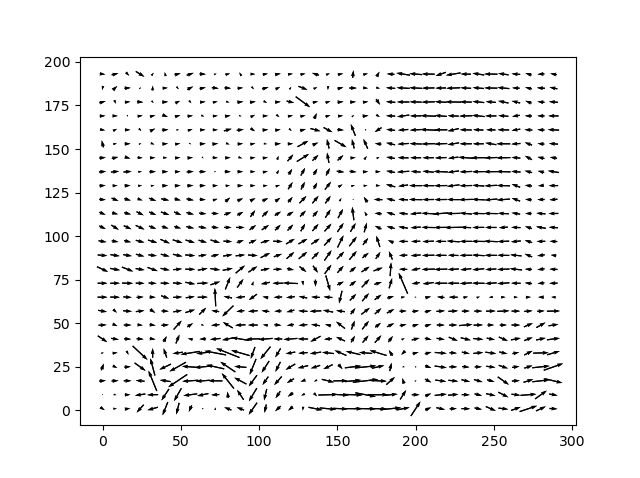
\includegraphics[height=30em]{prob4}
	\caption{Homography Splicing of Two Images}
	\label{fig:p4}
\end{figure*}

\solution{5}

\spart{a} In this problem we design a census transform, a representation of a local neighborhood of a pixel. The census transform encodes the number of pixels that are of lower intensity than the center pixel, with indices outside the boundary being considered 0 intensity. 

Since we are making a $5\times 5$ census transform, ie $\pm2$ pixels from the center, I padded the image with 2 zeros on each edge to avoid indexing problems. Then, I just loop through each pixel in the image, flattening the neighboring 24 pixels, and comparing them to the center. I used broadcasting of an array of $2^i$ multiplied by the boolean array of which pixels are less intensity to the center to get the census transform of the center pixel. 

\spart{b} In this problem we use the census transform coded in the previous to calculate an elementwise distance (hamming distance) between points on a horizontal line. By minimizing the hamming distance of between points in a left and right image we can get an estimate of depth in a pair of images. 

To do this we loop through every pixel, and test the hamming distance between $C_{left}[i,j]$ and $C_{right}[i,j-k]$ where $k=\{0,\dots,D_{max}\} $ and $D_{max}$ is the maximum horizontal distance we check. We then return the disparity of each pixel, this is shown in Figure \ref{fig:p5}.

\begin{figure*}[!h]
	\centering
	\includegraphics[height=15em]{prob5}
	\caption{Disparity Map of a Left and Right Image}
	\label{fig:p5}
\end{figure*}

%%%%%%%%%% Important, you must edit and complete the informational
%%%%%%%%%% section below. If you discussed the problem set with no
%%%%%%%%%% one, edit it to say no discussions or external resources.
\info

This problem set took approximately 20 hours of effort.

I discussed this problem set with no one.

% Note that you might have to escape some special symbols in URLS like \_
I also got hints from the following sources:
\begin{itemize}
\item Wikipedia article on binomial distribution at \url{https://en.wikipedia.org/wiki/Binomial_distribution}
%\item Read numpy tutorial from https://docs.scipy.org/doc/numpy-1.13.0/user/basics.broadcasting.html
\end{itemize}

\end{document}
